\documentclass[11pt]{article}
% Font tiếng việt
\usepackage{fontspec}
\usepackage[vietnamese]{babel}

% Sử dụng bảng dài có thể ngắt trang, ta cần thêm 2 gói này vào preamble
\usepackage{longtable}
\usepackage{ragged2e}
\usepackage{csquotes}       % Hỗ trợ quote
\usepackage[backend=biber, style=numeric-comp]{biblatex}
\addbibresource{references.bib}

\usepackage{graphicx}
\usepackage{amsmath, amssymb, amsfonts, bm}
\usepackage{xcolor}
\usepackage{hyperref}
\usepackage{pifont}
\newcommand{\xmark}{\ding{55}}
\newcommand{\cmark}{\ding{51}}
\usepackage{array}
\usepackage{float}


\definecolor{codehighlight}{rgb}{0.95,0.95,0.92} % Using your backcolour


\hypersetup{
    colorlinks=true,
    linkcolor=blue,
    filecolor=magenta,
    urlcolor=red,
    pdftitle={Overleaf Example},
    pdfpagemode=FullScreen,
}

\setmainfont{Times New Roman}
% \setsansfont{Arial} % Not used in the final layout, can comment out
% \setmonofont{Courier New} % Not used in the final layout, can comment out


% Page layout
\setlength{\topmargin}{-0.7in}
\setlength{\textheight}{9.25in}
\setlength{\oddsidemargin}{0in}
\setlength{\textwidth}{6.8in}

% No explicit title formatting needed as we'll place it manually
\usepackage{titling}
\setlength{\droptitle}{-10em} % Keep this to prevent default title spacing issues if using \maketitle later for other purposes

\renewcommand{\maketitle}{%
    \begin{center}
        \fontsize{18}{20}\selectfont\textbf{Module 3 Tuần 2  \\[0.2em] A Gentle Introduction to PySpark for Data Processing}\\[1em]
        \fontsize{14}{16}\selectfont Time-Series Team\\[0.5em]
        \fontsize{14}{16}\selectfont Ngày 10 tháng 8 năm 2025
    \end{center}
    \vspace{1.5em} % Add some space after the custom title block
}


% Remove fancy header/footer as it's not in the image
% \usepackage{fancyhdr}
% \pagestyle{fancy}
% \fancyhf{}
% \renewcommand{\footrulewidth}{0.4pt}
% \lhead{\bfseries AI VIETNAM}
% \rhead{\bfseries aivietnam.edu.vn}
% \fancyfoot[C]{\thepage}

% Section format (không đánh số section) - Keep this
\usepackage{titlesec}
\titleformat{\section}
{\normalfont\Large\bfseries}
{}{0em}{}

% Listings (code block) - Keep this if you plan to use code blocks
\usepackage{listings}
\definecolor{codegreen}{rgb}{0,0.6,0}
\definecolor{codegray}{rgb}{0.5,0.5,0.5}
\definecolor{codepurple}{rgb}{0.58,0,0.82}
\definecolor{backcolour}{rgb}{0.95,0.95,0.92}
\lstdefinestyle{mystyle}{
    backgroundcolor=\color{backcolour},
    commentstyle=\color{codegreen},
    keywordstyle=\color{magenta},
    numberstyle=\tiny\color{codegray},
    stringstyle=\color{codepurple},
    basicstyle=\ttfamily\footnotesize,
    breaklines=true,
    captionpos=b,
    keepspaces=true,
    numbers=left,
    numbersep=5pt,
    tabsize=2,
    showspaces=false,
    showstringspaces=false,
    showtabs=false
}
\lstset{style=mystyle}


% Colored boxes
\usepackage[many]{tcolorbox}
\definecolor{lightgreenbox}{rgb}{0.85,0.95,0.85} % A light green color closer to the image
\newtcolorbox{summarybox}{
    colback = lightgreenbox,
    colframe = green!50!black, % A slightly darker green border
    boxsep = 5pt,
    arc = 4pt,
    outer arc = 4pt,
    boxrule = 0.5pt,
    left = 10pt,
    right = 10pt,
    top = 10pt,
    bottom = 10pt,
    % Add this line to ensure proper font encoding for Vietnamese characters
    fontupper = \setmainfont{Times New Roman}\normalfont,
}

% For math proofs or custom counters (tuỳ chọn nếu cần) - Can be removed if not used
\usepackage{lipsum}
\newcounter{mycounter}
\newcommand\showmycounter{\stepcounter{mycounter}\themycounter}
\newcommand\showlips{\stepcounter{mycounter}\lipsum[\value{mycounter}]}

% Others - Can be removed if not used
\usepackage{booktabs}
\usepackage{subcaption}
\usepackage{framed}
\usepackage{tikz}


%%%%%%%%%%%%%%%%%%%%%%%%%%%%%%%%%%%%%%%%%%%%%%%%%%%%%%%%%%%%%%%%%%%%%%%%%%%%%
%%%%%%%%%%%%%%%%%%%%%%%%%%%%%%%%%%%%%%%%%%%%%%%%%%%%%%%%%%%%%%%%%%%%%%%%%%%%%
%%%%%%%%%%%%%%%%%%%%%%%%%%%%%%%%%%%%%%%%%%%%%%%%%%%%%%%%%%%%%%%%%%%%%%%%%%%%%
\begin{document}


\maketitle % Call the redefined maketitle to display the custom title and date

\begin{summarybox}
   Buổi học thứ 5 (ngày 7/8/2025) được chia thành 4 phần chính nhằm giúp ta hiểu được Cách PySpark xử lý dữ liệu cho Big Data và Machine Learning:
    \begin{itemize}
        \item \textbf{Phần 1: Big Data là gì và vì sao lại cần nó}
        \item \textbf{Phần 2: Giải thích cơ chế hoạt động của Hadoop và Apache Spark}
        \item \textbf{Phần 3: Pyspark trong Python và SQL}
        \item \textbf{Phần 4:  So sánh workflow của Sklearn và PySpark để dễ hiểu hơn}
    \end{itemize}
\end{summarybox}

\section{Phần 1: Big Data là gì và vì sao lại cần nó}
\section{Vì sao lại cần Big Data trong thế giới hiện nay?}
Khối lượng dữ liệu toàn cầu dự kiến sẽ đạt khoảng \textbf{180--163 zettabyte} vào năm 2025 \cite{idc2023}, để hình dung thì 1 chiếc điện thoại ngày nay có 128GB và 1 zettabytes bằng 1 nghìn tỷ GB, tương đương với 7.8 tỷ chiếc điện thoại. Vậy nên việc xử lý, thu thập và xử lý thông tin lớn như BigData hay không, không phải là 1 lựa chọn mà là \textbf{1 lĩnh vực bắt buộc phải hiểu} để không bị bỏ lại phía sau.

\medskip
\noindent Để dễ hình dung, ví dụ khi ta viết một chương trình nhỏ để tìm kiếm tên ta trong danh sách 100 người, thì việc xử lý khá đơn giản --- đọc dữ liệu, tìm tên, trả kết quả.

Nhưng nếu:
\begin{itemize}
    \item Dữ liệu không phải 100 người, mà là \textbf{100 triệu bản ghi} (hoặc hơn).
    \item Dữ liệu nằm rải rác ở nhiều nơi: server ở Hà Nội, TP.HCM, Singapore...
    \item Dữ liệu có nhiều kiểu và một trong số đó còn là thông tin chưa được xử lý.
    \item Yêu cầu phải trả kết quả \textbf{trong vài giây}.
\end{itemize}

Lúc này, ta sẽ gặp hai lớp vấn đề:

\paragraph{Lớp 1 -- Logic của chương trình:}
Đây là ``bộ não'' của ứng dụng:
\begin{itemize}
    \item Xác định ứng dụng cần làm gì (tìm kiếm, lọc, tính toán...).
    \item Viết bằng ngôn ngữ như Python, Java, SQL,...
    \item Ví dụ: ``Tìm tất cả khách hàng đã mua hàng trên 5 triệu đồng trong tháng 7''.
\end{itemize}

\paragraph{Lớp 2 -- Thực thi trên dữ liệu khổng lồ:}
Đây là phần khó khi dữ liệu rất lớn:
\begin{itemize}
    \item \textbf{Chia nhỏ dữ liệu} để xử lý song song.
    \item \textbf{Phân việc} cho nhiều máy chủ khác nhau.
    \item \textbf{Tối ưu hạ tầng} để mọi máy hoạt động trơn tru.
    \item \textbf{Tổng hợp kết quả} từ nhiều máy và trả về cho người dùng.
    \item \textbf{Xử lý lỗi}: nếu một máy hỏng, hệ thống vẫn tiếp tục chạy.
\end{itemize}

\noindent\textit{Như khi ta tra cứu  Google}, không phải một máy tính duy nhất tìm kiếm toàn bộ Internet. Hàng trăm máy sẽ chạy song song, mỗi máy xử lý một phần dữ liệu, rồi kết quả được gom lại cực nhanh.



% \begin{itemize}
% \item Lớp 1 là logic của chính chương trình đấy
% \item Lớp 2 là việc thực thi logic ấy trên 1 bộ dữ liệu khổng lồ mà vẫn đảm bảo hiệu năng. Ví dụ 1 hàm search trên 1 kho dữ liệu khổng lồ là không đơn giản. Các giải pháp song song trên BigData phải phân tích nhiệm vụ, chia thành các tác vụ, chia việc cho các cụm máy, quản lý tài nguyên, gom góp kết quả, tổng hợp kết quả, tối ưu hạ tầng, phần cứng cho 1 lệnh tưởng chừng rất đơn giản.
% \end{itemize}

% Những giải pháp như Spark theo mình nghĩ là đảm bảo làm sao mình chủ yếu quan tâm đến công việc lớp 1 và không phải quan tâm đến quá nhiều công việc ở lớp 2. Đi vào chi tiết thì hoa mắt nhưng hiểu sơ sơ thì vậy.

\subsection{Big Data là gì ?}
Dữ liệu trở thành Big Data khi đạt đủ 5 tiêu chí \textbf{5V}):
\begin{enumerate}
    \item \textbf{Volume} -- Khối lượng dữ liệu khổng lồ. \\
    \textit{Ví dụ:} Facebook lưu trữ hàng tỷ bức ảnh.
    \item \textbf{Velocity} -- Tốc độ dữ liệu được tạo ra và xử lý. \\
    \textit{Ví dụ:} Dữ liệu livestream, giao dịch ngân hàng theo thời gian thực.
    \item \textbf{Variety} -- Sự đa dạng về định dạng và nguồn dữ liệu, dữ liệu có cấu trúc hoặc không hoặc bán cấu trúc. \\
    \textit{Ví dụ:} Văn bản, video, ảnh, log server.
    \item \textbf{Veracity} --Độ tin cậy và tính chính xác của dữ liệu. \\
      \textit{Ví dụ:} Bộ dữ liệu y tế có thể chứa thông tin nhập sai hoặc trùng lặp.

    \item \textbf{Value} -- Giá trị mà dữ liệu đó mang lại. \\
    \textit{Ví dụ:}
	\begin{itemize}
		\item Cải thiện trải nghiệm khách hàng qua phân tích hành vi mua hàng để gợi ý sản phẩm phù hợp cho từng khách hàng.
		\item Giảm chi phí qua phân tích những vấn đè, yếu tố lớn nhất đang kéo doanh thu xuống mà không mang lại lợi ích gì.
		\item Giải quyết vấn đề tốt hơn qua hình dung vấn đề trong dữ liệu.
		\item Gia tăng lợi nhuận nhờ vào phân tích mảng khách hàng cần quan tâm.
	\end{itemize}

\end{enumerate}

\subsection{Tại sao cần các giải pháp như Apache Spark?}
Các nền tảng như \textbf{Apache Spark} cho phép lập trình viên:
\begin{itemize}
    \item Tập trung vào \textbf{Lớp 1} (logic xử lý) thay vì tự viết toàn bộ \textbf{Lớp 2}.
    \item Tự động chia dữ liệu và phân công cho nhiều máy xử lý.
    \item Quản lý tài nguyên và tổng hợp kết quả.
    \item Hỗ trợ cả dữ liệu \textbf{batch} và \textbf{streaming} (thời gian thực).
\end{itemize}

\noindent\textit{Nói cách khác:} ta chỉ cần ``ra mệnh lệnh'' và Spark sẽ huy động ``đội quân máy tính'' để làm phần còn lại.


\section{Phần 2: Giải thích cơ chế hoạt động của Hadoop và Apache Spark}

\subsection{Mục Đích của Hadoop và Apache Spark}
Từ ví dụ ở phần trước, khi khối lượng dữ liệu lên đến hàng trăm triệu bản ghi, phân tán ở nhiều máy chủ và yêu cầu phản hồi trong vài giây, ta cần đến các \textit{framework} xử lý dữ liệu phân tán.
\begin{figure}[H]
    \centering
    \includegraphics[width=0.7\linewidth]{HadoopPysparkComparison.png}
    \caption{Hadoop and Apache comparison}
\end{figure}
\begin{itemize}
    \item \textbf{Hadoop} phù hợp với \textit{batch processing} khối lượng lớn, tận dụng mô hình \textbf{HDFS + MapReduce} để \textbf{lưu trữ và xử lý dữ liệu theo Batch}.
    \item \textbf{Apache Spark} kế thừa và mở rộng ý tưởng từ Hadoop, sử dụng \textit{in-memory computing} giúp xử lý nhanh hơn, hỗ trợ cả \textit{batch} và \textit{streaming} dữ liệu, thuận tiện hơn cho \textbf{phân tích dữ liệu thời gian thực.}
\end{itemize}

\begin{figure}[H]
    \centering
    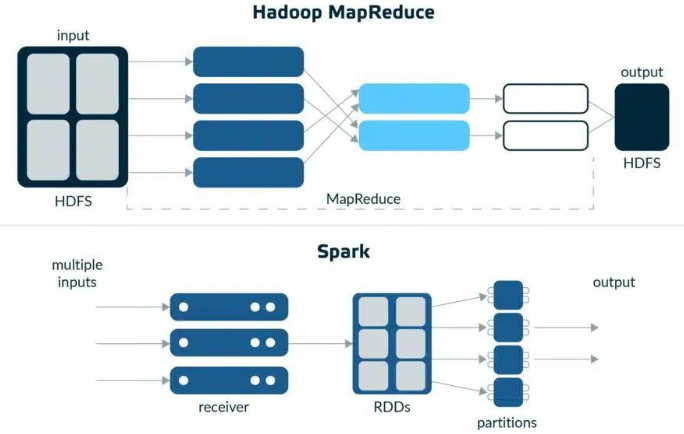
\includegraphics[width=0.7\linewidth]{hd_vs_sp.png}
    \caption{Minh họa workflow của Hadoop và Spark}
\end{figure}

Tóm lại, để xử lý dữ liệu lớn ta cần 1 hệ thống chuyển lưu trữ rồi xử lý dữ liệu theo Batch và 1 hệ thống cho phép phân tích dữ liệu theo thời gian thực sử dụng RAM. Giống như Ổ Cứng và RAM trong máy tính.


\subsection{HDFS (Hadoop Distributed File System)}
HDFS là hệ thống lưu trữ phân tán được thiết kế để xử lý dữ liệu lớn trên nhiều máy chủ.
Toàn bộ workflow của HDFS có thể tóm tắt như sau: khi \textbf{HDFS Client gửi yêu cầu đọc hoặc ghi dữ liệu},
HDFS Client sẽ \text{giao tiếp với NameNode để lấy metadata} (cơ bản nó là 1 json string chứa chứa nhiều cặp keys và values)
và \text{thông tin vị trí các block} dữ liệu xanh đỏ tím vàng như minh họa. Sau đó, \textbf{Client giao tiếp trực tiếp với các DataNode}
để lấy hoặc ghi dữ liệu. Lưu ý là các block được nhân bản (replication) trên nhiều DataNode để đảm bảo dữ liệu vẫn khả dụng ngay cả khi một máy bị hỏng.

\begin{figure}[H]
    \centering
    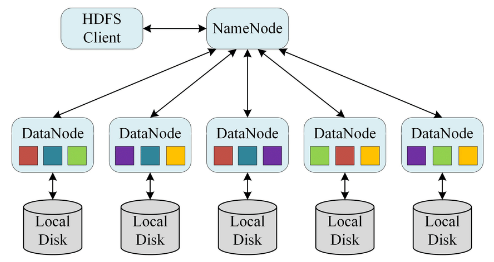
\includegraphics[width=0.7\linewidth]{hdfs.png}
    \caption{Cấu trúc HDFS}
    \label{fig:hdfs-structure}
\end{figure}

\noindent Các thành phần chính:
\begin{itemize}
    \item \textbf{NameNode}: ``Bộ não'' của HDFS, quản lý metadata, vị trí các block, và điều phối việc đọc/ghi.
    \item \textbf{DataNode}: Lưu trữ dữ liệu thực tế dưới dạng block, mỗi DataNode chạy trên một máy chủ riêng.
    \item \textbf{HDFS Client}: Gửi yêu cầu đến NameNode và truy cập dữ liệu từ DataNode.
    \item \textbf{Replication}: Mỗi block được nhân bản trên nhiều DataNode để tăng khả năng chịu lỗi và độ sẵn sàng.
\end{itemize}



\subsection{MapReduce}
MapReduce là mô hình xử lý dữ liệu lớn theo cơ chế chia nhỏ và tổng hợp. Workflow tổng quát: dữ liệu đầu vào được chia nhỏ (\textbf{Splitting}) thành nhiều phần và xử lý song song bởi các hàm \texttt{Map}, tạo ra các cặp \texttt{(key, value)}. Sau đó, hệ thống thực hiện \textbf{Shuffling} để nhóm các giá trị cùng key lại với nhau, và cuối cùng \texttt{Reduce} tổng hợp chúng để tạo ra kết quả cuối cùng.
\begin{figure}[H]
    \centering
    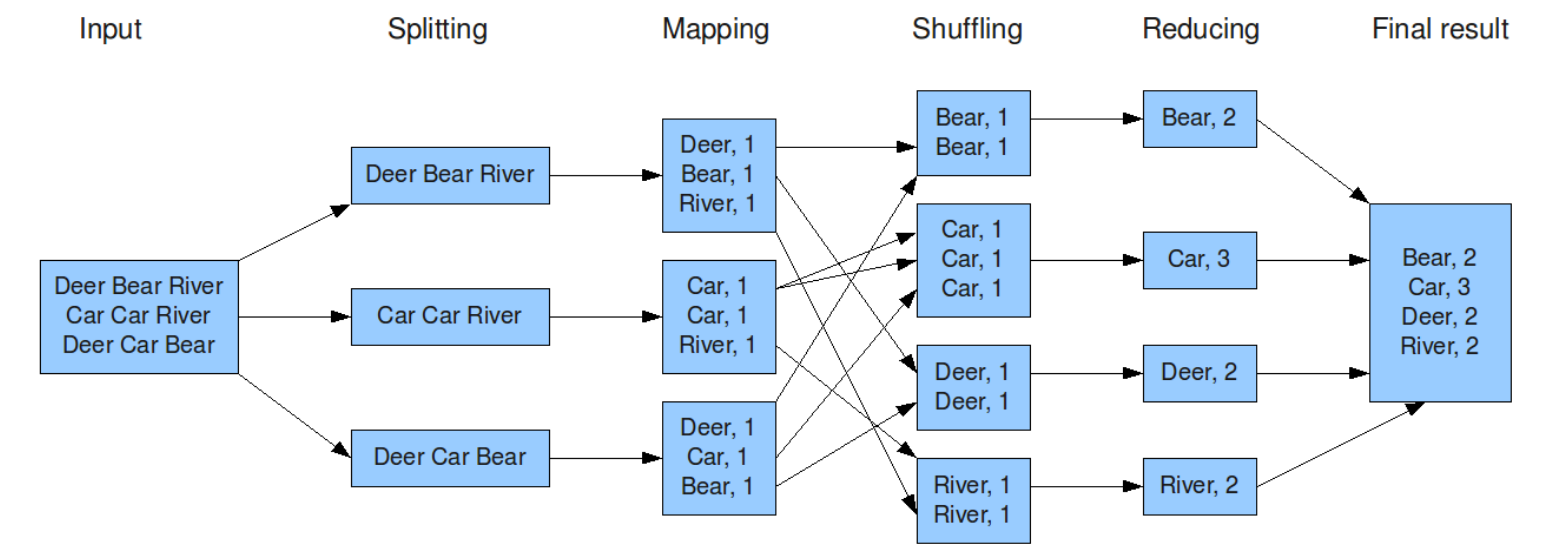
\includegraphics[width=0.9\linewidth]{mapReduce.png}
    \caption{Quy trình MapReduce}
    \label{fig:mapreduce-flow}
\end{figure}

\noindent Ví dụ các bước lưu trữ thông tin qua ví dụ đếm số chữ, giống `token\_dict`' trong NLP:
\begin{enumerate}
    \item \textbf{Splitting}: Chia dữ liệu thành các chunk nhỏ để xử lý song song.
    \item \textbf{Mapping}: Hàm \texttt{Map} xử lý từng chunk và phát ra các cặp \texttt{(key, value)}.
    \item \textbf{Shuffling}: Gom nhóm các giá trị có cùng \texttt{key}.
    \item \textbf{Reducing}: Hàm \texttt{Reduce} xử lý từng nhóm \texttt{key} để tạo kết quả.
    \item \textbf{Final Result}: Tổng hợp và xuất ra kết quả cuối cùng.
\end{enumerate}



\subsection{Tổng quan Pipeline hoạt động của Apache Spark}
Để hiểu rõ hơn Apache Spark có hoạt động như thế nào, mình sẽ đi qua 1 workflow xử lý dữ liệu cho Học Máy,
Flow bắt đầu từ việc thu thập dữ liệu từ nhiều nguồn khác nhau (streaming: dữ liệu được cập nhật liên tục và static: dữ liệu đã lưu),
sau đó xử lý bằng các API như DataFrame hoặc Spark SQL, thực hiện các tác vụ phân tích nâng cao (MLlib),
và cuối cùng lưu trữ kết quả (i.e. dữ liệu đã xử lý) vào các hệ thống lưu trữ dữ liệu.

\begin{figure}[H]
    \centering
    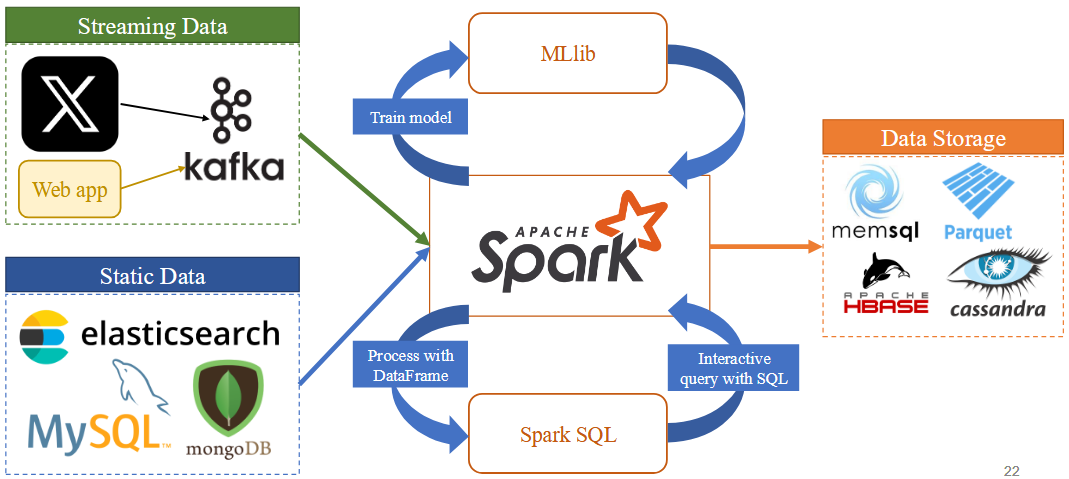
\includegraphics[width=0.9\linewidth]{PySpark_pipeline.png}
    \caption{Pipeline xử lý dữ liệu với PySpark}
    \label{fig:pyspark-pipeline}
\end{figure}

\noindent Các bước chính trong pipeline:
\begin{enumerate}
    \item \textbf{Streaming Data}: Thu thập dữ liệu thời gian thực từ các nguồn như Kafka (ví dụ: dữ liệu mạng xã hội, log từ web app).
    \item \textbf{Static Data}: Đọc dữ liệu tĩnh từ các hệ quản trị cơ sở dữ liệu hoặc công cụ tìm kiếm như Elasticsearch, MySQL, MongoDB.
    \item \textbf{Process with DataFrame}: Sử dụng API DataFrame của Spark để xử lý dữ liệu một cách linh hoạt và tối ưu, tận dụng khả năng \textit{in-memory computing}.
    \item \textbf{Spark SQL}: Thực hiện các truy vấn tương tác với dữ liệu thông qua cú pháp SQL.
    \item \textbf{MLlib}: Áp dụng các thuật toán học máy như phân loại, hồi quy, clustering để phân tích và trích xuất thông tin.
    \item \textbf{Data Storage}: Lưu kết quả phân tích vào các hệ thống lưu trữ phân tán như MemSQL, Apache HBase, Cassandra hoặc định dạng file tối ưu như Parquet.
\end{enumerate}




\subsection{Pyspark Ecosystem}
Để vận hành và xử ý dữ liệu trơn tru cho các mục đích khác nhau, các hệ sinh thái được xây dựng lên xung quanh Apache Spark:
\begin{itemize}
\item Storage and Infrastructure đóng vai trò là "nền móng", nơi lưu trữ và quản lý dữ liệu khổng lồ (ví dụ: Hadoop, S3, Parquet).
\item Data Science and Machine Learning là "công cụ" để các Data Scientist xây dựng các mô hình phức tạp, phân tích dữ liệu chuyên sâu và trích xuất thông tin giá trị từ dữ liệu thô/raw.
\item SQL Analytics and BI là "giao diện", nơi dữ liệu đã được xử lý và phân tích được trình bày dưới dạng trực quan, giúp khách hàng dễ dàng hiểu và đưa ra quyết định. \\
\end{itemize}

\noindent Lưu ý: mô tả thư viện dưới đây chỉ mang tính chất tham khảo, để hiểu chỉ cần đọc mô tả của từng phần. \\
\noindent \textbf{Data science and Machine learning:} sử dụng để mở rộng khả năng xử lý dữ liệu lớn bằng cách tích hợp các mô hình và thuật toán học máy.
\begin{itemize}
\item \href{https://scikit-learn.org/stable/}{scikit-learn}: Một bộ công cụ dành cho lập trình viên Python để xây dựng các mô hình học máy một cách đơn giản, ví dụ như dự đoán xu hướng hoặc phân loại dữ liệu.
\item \href{https://pandas.pydata.org/}{pandas}: Giống như một bảng tính Excel siêu mạnh trong Python, giúp ta dễ dàng làm sạch, xử lý và phân tích dữ liệu.
\item \href{https://www.tensorflow.org/}{TensorFlow}: Một nền tảng mạnh mẽ giúp ta tạo ra các mô hình học máy phức tạp, đặc biệt là các mô hình sử dụng mạng lưới nơ-ron để làm những việc như nhận diện hình ảnh hoặc dịch ngôn ngữ.
\item \href{https://pytorch.org/}{PyTorch}: Một công cụ khác, cũng rất phổ biến để xây dựng các mô hình học máy, được nhiều nhà nghiên cứu ưa chuộng vì tính linh hoạt và dễ sử dụng.
\item \href{https://mlflow.org/}{mlflow}: Một công cụ giúp ta quản lý toàn bộ quá trình phát triển các mô hình học máy, từ việc thử nghiệm các thuật toán khác nhau cho đến khi triển khai chúng.
\item \href{https://www.r-project.org/}{R}: Một ngôn ngữ lập trình chuyên biệt dành cho các nhà thống kê và nhà khoa học dữ liệu để phân tích dữ liệu và tạo ra các biểu đồ đẹp mắt.
\item \href{https://numpy.org/}{NumPy}: Nền tảng cơ bản cho hầu hết các thư viện khoa học dữ liệu trong Python, giúp xử lý các phép toán với số và ma trận một cách cực kỳ nhanh chóng.
\end{itemize}

\noindent\textbf{SQL analytics and BI:} dùng để trực quan hóa và phân tích dữ liệu đã được xử lý hoặc lưu trữ, giúp tạo ra báo cáo và bảng điều khiển hữu ích.

\begin{itemize}
\item \href{https://superset.apache.org/}{Apache Superset}: Một công cụ mã nguồn mở giúp ta tạo ra các bảng điều khiển (dashboard) và biểu đồ tương tác để khám phá dữ liệu của mình mà không cần phải viết nhiều code.
\item \href{https://powerbi.microsoft.com/en-us/}{Power BI}: Một dịch vụ của Microsoft giúp ta biến dữ liệu thô thành những báo cáo và biểu đồ dễ hiểu, giúp ta đưa ra quyết định kinh doanh tốt hơn.
\item \href{https://looker.com/}{Looker}: Một nền tảng phân tích dữ liệu giúp các công ty dễ dàng truy cập và hiểu dữ liệu của họ, đặc biệt là khi dữ liệu phức tạp.
\item \href{https://redash.io/}{re:dash}: Một công cụ mã nguồn mở giúp ta tạo các bảng điều khiển trực quan và chia sẻ kết quả truy vấn dữ liệu với đồng nghiệp.
\item \href{https://www.tableau.com/}{tableau}: Một trong những công cụ hàng đầu trong việc trực quan hóa dữ liệu, giúp ta tạo ra những biểu đồ và đồ thị tương tác một cách nhanh chóng.
\item \href{https://www.getdbt.com/}{dbt}: Một công cụ dành cho các kỹ sư dữ liệu để biến đổi dữ liệu thô trong kho dữ liệu thành các bảng đã được làm sạch và chuẩn bị sẵn sàng cho việc phân tích.
\end{itemize}

\noindent\textbf{Storage and Infrastructure:} đóng vai trò quan trọng trong việc lưu trữ, quản lý và xử lý dữ liệu lớn, tạo nền tảng vững chắc cho các tác vụ phân tích và học máy.

\begin{itemize}
\item \href{https://www.elastic.co/}{elasticsearch}: Giống như một công cụ tìm kiếm Google cho dữ liệu của ta, giúp ta tìm kiếm thông tin một cách nhanh chóng và mạnh mẽ.
\item \href{https://www.mongodb.com/}{mongoDB}: Một loại cơ sở dữ liệu linh hoạt, không cần tuân theo cấu trúc bảng cố định như Excel, rất phù hợp để lưu trữ dữ liệu đa dạng như thông tin người dùng trên mạng xã hội.
\item \href{https://kafka.apache.org/}{Apache Kafka}: Một "ống dẫn" dữ liệu tốc độ cao, dùng để chuyển tiếp một lượng lớn dữ liệu theo thời gian thực từ nhiều nguồn khác nhau đến nơi cần xử lý.
\item \href{https://airflow.apache.org/}{Apache Airflow}: Một công cụ để lên lịch và quản lý các công việc phức tạp, giúp ta đảm bảo các quy trình xử lý dữ liệu luôn chạy đúng thứ tự và đúng thời điểm.
\item \href{https://parquet.apache.org/}{Parquet}: Một cách để lưu trữ dữ liệu hiệu quả, đặc biệt là khi ta chỉ cần truy cập một vài cột dữ liệu trong một tập tin lớn.
\item \href{https://www.microsoft.com/en-us/sql-server}{Microsoft SQL Server}: Một hệ thống quản lý cơ sở dữ liệu truyền thống, rất mạnh mẽ và ổn định, được sử dụng rộng rãi trong các doanh nghiệp.
\item \href{https://delta.io/}{Delta Lake}: Một "lớp phủ" giúp cải thiện độ tin cậy và hiệu suất của các kho dữ liệu lớn, giúp dữ liệu luôn nhất quán và dễ quản lý hơn.
\item \href{https://kubernetes.io/}{kubernetes}: Một công cụ giúp ta quản lý hàng trăm, thậm chí hàng ngàn, ứng dụng nhỏ (gọi là container) một cách tự động, đảm bảo chúng luôn chạy ổn định.
\item \href{http://cassandra.apache.org/}{cassandra}: Một loại cơ sở dữ liệu phân tán, được thiết kế để xử lý lượng dữ liệu khổng lồ trên nhiều máy chủ mà không bao giờ bị lỗi.
\item \href{https://orc.apache.org/}{Apache ORC}: Một định dạng lưu trữ dữ liệu khác, tương tự Parquet, cũng giúp tối ưu hóa việc truy cập và xử lý dữ liệu.
\end{itemize}


\subsection{Kiến trúc của Apache Spark}
Phần này mô tả workflow tổng quát của Spark theo kiến trúc top-down: bắt đầu từ \textbf{Spark Driver} gửi công việc xuống các \textbf{Spark Worker}, mỗi worker gắn với một \textbf{Data Node} lưu dữ liệu trên \textbf{Hadoop HDFS}. Tại mỗi worker, dữ liệu được xử lý bởi \textbf{Executor} thông qua các \textbf{Task} thực thi trên các \textbf{Partition} dữ liệu.

\begin{figure}[H]
    \centering
    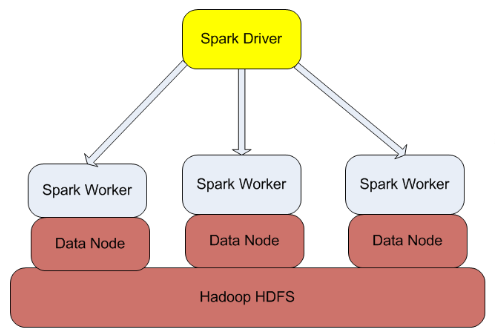
\includegraphics[width=0.65\linewidth]{pySpark_highlevel.png}
    \caption{PySpark top-down architecture}
\end{figure}

\paragraph{Workflow tổng quát.}
\begin{enumerate}
    \item \textbf{Spark Driver} khởi tạo ứng dụng, xây dựng kế hoạch xử lý (job) và gửi yêu cầu tới các \textbf{Spark Worker}.
    \item Mỗi \textbf{Spark Worker} liên kết với một \textbf{Data Node} để truy xuất dữ liệu từ \textbf{HDFS}.
    \item Worker khởi chạy \textbf{Executor}, chia dữ liệu thành các \textbf{Partition} và gán \textbf{Task} cho từng partition.
    \item Các Task chạy song song trên nhiều node, sau đó trả kết quả về Spark Driver hoặc ghi ra storage.
\end{enumerate}

\paragraph{Thành phần chính.}
\begin{itemize}
    \item \textbf{Spark Driver}: Điều phối toàn bộ luồng xử lý.
    \item \textbf{Spark Worker}: Node tính toán, nhận lệnh từ Driver.
    \item \textbf{Executor}: Tiến trình trên Worker thực hiện các Task.
    \item \textbf{Data Node}: Nơi lưu trữ dữ liệu vật lý, thường là các block trong HDFS.
    \item \textbf{HDFS}: Hệ thống lưu trữ phân tán cung cấp dữ liệu cho Spark.
\end{itemize}

\begin{figure}[H]
    \centering
    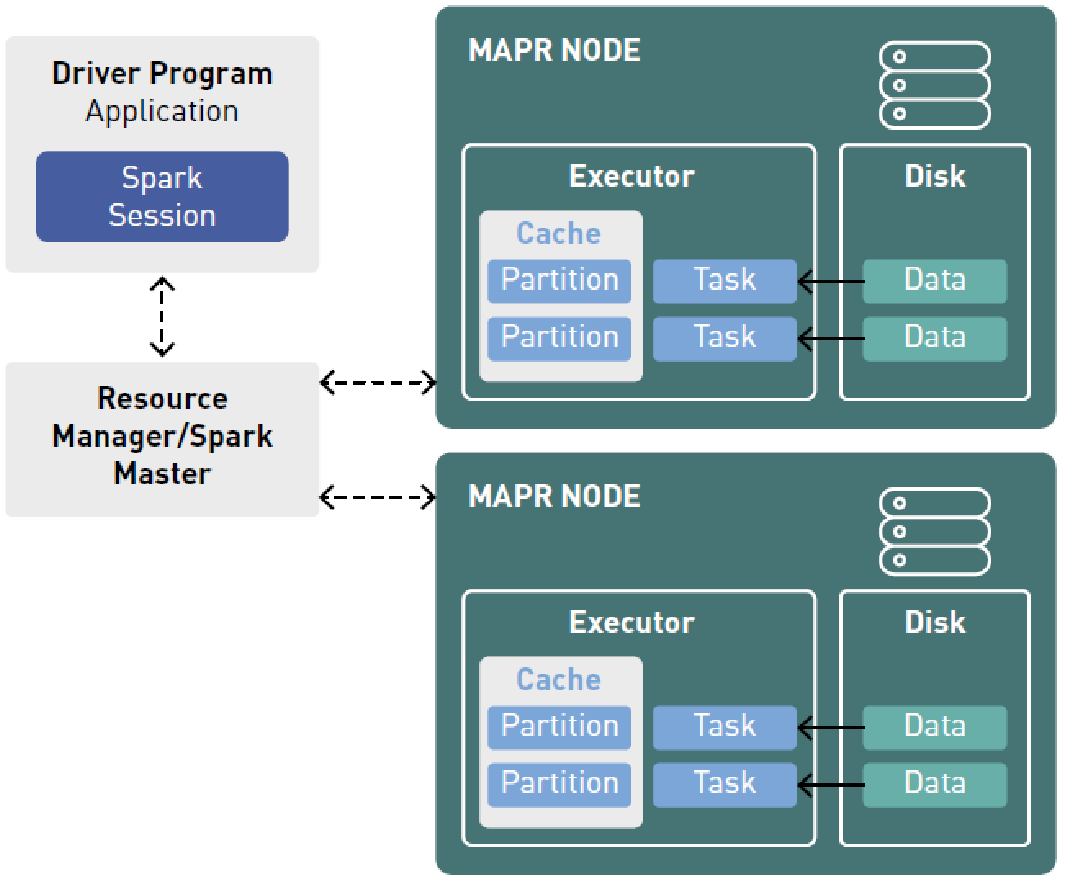
\includegraphics[width=0.75\linewidth]{SparkSystemOverview.png}
    \caption{Ví dụ chi tiết kiến trúc Spark: Driver, Resource Manager, Executors và Data Nodes}
\end{figure}

\subsection{Apache Spark: RDD (Resilient Distributed Dataset)}
RDD là cấu trúc dữ liệu cốt lõi của Spark, được phân tán (\textbf{Distributed}) qua nhiều node, có khả năng chịu lỗi (\textbf{Resilient}) và chứa dữ liệu dưới dạng các \textbf{Partition}. Phần này mô tả workflow RDD từ khi dữ liệu nằm trên \textbf{Disk/HDFS} đến khi được xử lý trong \textbf{RAM} thông qua các \textbf{Transformations}.

\begin{figure}[H]
    \centering
    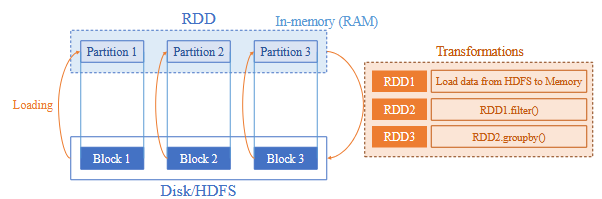
\includegraphics[width=0.9\linewidth]{pysparkRDD.png}
    \caption{PySpark RDD: Partition từ Disk/HDFS và xử lý In-memory}
\end{figure}

\paragraph{Workflow tổng quát.}
\begin{enumerate}
    \item \textbf{Loading}: Dữ liệu được đọc từ \textbf{Disk/HDFS} dưới dạng các \textbf{Block}.
    \item Mỗi Block trong ổ cứng ánh xạ thành một \textbf{Partition} trong RDD và được load vào \textbf{In-memory (RAM)}.
    \item Các \textbf{Transformations} (ví dụ: \texttt{filter()}, \texttt{groupBy()}) được áp dụng lên partition nhưng chỉ lưu dưới dạng lineage (lazy) - nghĩa là Spark lưu lại lịch sử thực thi chứ chưa thực thi ngay.

    \medskip
    Dựa trên \textbf{lineage}, Spark xây dựng một \textbf{DAG} (Directed Acyclic Graph) thể hiện mối quan hệ phụ thuộc giữa các bước xử lý. DAG là \textit{kế hoạch thực thi} được Spark tối ưu hóa trước khi chạy, giúp:
    \begin{itemize}
        \item Xác định thứ tự các phép tính cần thực hiện.
        \item Chia công việc thành các \textbf{stage} và \textbf{task} để xử lý song song.
        \item Tái tính toán dữ liệu nếu một partition bị mất, bằng cách chạy lại các bước cần thiết trong DAG.
    \end{itemize}

    \textrightarrow \space Nói chung, lineage được tạo ra để lưu lịch sử thực thi và DAG được tạo ra để nắm bắt mqh giữa các bước thực thi dể khi chạy lỗi sẽ không phải chạy lại.

    \item Khi gặp một \textbf{Action} (ví dụ: \texttt{count()}, \texttt{collect()}), Spark thực thi pipeline: chia thành \textbf{Tasks} chạy song song trên các partition.
    \item Kết quả được trả về hoặc ghi lại xuống storage; các partition có thể được \textbf{Cache} để tái sử dụng.
\end{enumerate}

\paragraph{Thành phần chính.}
\begin{itemize}
    \item \textbf{Block}: Đơn vị lưu trữ của HDFS.
    \item \textbf{Partition}: Đơn vị tính toán song song của Spark, ánh xạ từ Block.
    \item \textbf{In-memory (RAM)}: Nơi Spark giữ partition đã load để giảm I/O.
    \item \textbf{Transformations}: Các phép biến đổi tạo RDD mới một cách lazy.
    \item \textbf{Actions}: Kích hoạt thực thi và trả kết quả.
\end{itemize}


\section{Phần 3: PySpark trong Python và SQL}
Phần này trình bày các \textbf{component} chính của PySpark và cách chúng tích hợp Spark SQL và Spark MLlib trong xử lý dữ liệu phân tán.

\subsection{Spark SQL}
\textbf{Spark SQL} tích hợp truy vấn SQL với sức mạnh xử lý phân tán của Spark:
\begin{itemize}
    \item Hỗ trợ nhiều định dạng dữ liệu: Parquet, JSON, CSV, Elasticsearch, JDBC.
    \item DataFrame cung cấp API thống nhất để làm việc với dữ liệu có cấu trúc và bán cấu trúc.
    \item Workflow: Load dữ liệu $\rightarrow$ xử lý truy vấn với SQL $\rightarrow$ xuất DataFrame kết quả.
\end{itemize}

\subsection{Spark MLlib}
\textbf{Spark MLlib} cung cấp thư viện Machine Learning phân tán:
\begin{itemize}
    \item Thuật toán: classification, regression, clustering, collaborative filtering.
    \item Feature engineering: feature extraction, transformation, dimensionality reduction.
    \item ML Pipeline: ingest dữ liệu $\rightarrow$ tiền xử lý $\rightarrow$ huấn luyện mô hình $\rightarrow$ kiểm thử $\rightarrow$ deploy.
\end{itemize}

\subsection{PySpark Layers}
PySpark được thiết kế theo hai tầng chính:
\begin{figure}[H]
    \centering
    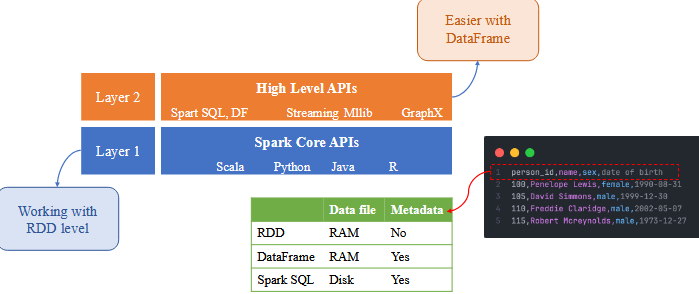
\includegraphics[width=0.65\linewidth]{pysparkLayer.png}
    \caption{PySpark Layer}
    \label{fig:pyspark_layer}
\end{figure}

\begin{itemize}
    \item \textbf{Layer 1 -- Spark Core APIs:} Cung cấp API nền tảng cho nhiều ngôn ngữ (Scala, Python, Java, R). Ở mức này, lập trình viên làm việc trực tiếp với \textbf{RDD} (Resilient Distributed Dataset) - viết hàm, tập trung vào các thao tác low-level như \texttt{map()}, \texttt{filter()}, \texttt{reduceByKey()}, hoặc 1 Custom RDD.
    \item \textbf{Layer 2 -- High Level APIs:} Bao gồm các API nâng cao như \textbf{Spark SQL / DataFrame}, \textbf{Spark Streaming}, \textbf{MLlib}, \textbf{GraphX} giúp đơn giản hóa việc xử lý dữ liệu bằng cách cung cấp cú pháp dễ đọc, hỗ trợ metadata, và tích hợp nhiều chức năng xử lý dữ liệu.
\end{itemize}
So sánh:
\begin{itemize}
    \item \textbf{RDD:} Lưu dữ liệu trong RAM, không có metadata.
    \item \textbf{DataFrame:} Lưu dữ liệu trong RAM, có metadata (schema), tối ưu cho truy vấn và thao tác dạng bảng.
    \item \textbf{Spark SQL:} Lưu trên disk, có metadata, thích hợp cho phân tích dữ liệu lớn với truy vấn SQL.
\end{itemize}


\subsection{PySpark RDD}
\textbf{RDD} là cấu trúc dữ liệu nền tảng của Spark, biểu diễn tập dữ liệu phân tán, có khả năng chịu lỗi, và bất biến (immutable). Mỗi \textbf{RDD} có thể được xem như một \textit{function} áp dụng lên dữ liệu đầu vào.
\begin{enumerate}
    \item \textbf{Transformations:} (ví dụ: \texttt{map()}, \texttt{filter()}, \texttt{flatMap()}, \texttt{union()}) — tạo ra một RDD mới từ RDD gốc, nhưng không thực thi ngay (lazy evaluation). Spark lưu lại lịch sử thực thi (lineage) để tối ưu và phục hồi dữ liệu khi cần.
    \item \textbf{Actions:} (ví dụ: \texttt{count()}, \texttt{collect()}, \texttt{saveAsTextFile()}) — kích hoạt việc thực thi pipeline các transformations và trả về kết quả.
\end{enumerate}

\begin{figure}[H]
    \centering
    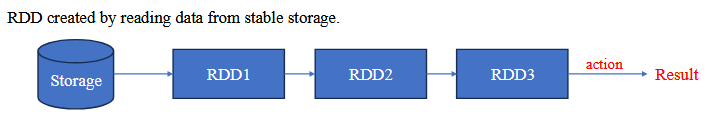
\includegraphics[width=0.7\linewidth]{pysparkRDD_code.png}
    \caption{PySpark RDD Workflow in Code}
\end{figure}

\noindent
Ví dụ code minh họa:
\begin{verbatim}
# Tạo SparkContext
from pyspark import SparkContext
sc = SparkContext("local", "RDD Example")

# Tạo RDD từ list Python
data = [1, 2, 3, 4, 5]
rdd = sc.parallelize(data)

# Transformation: nhân đôi mỗi phần tử
rdd2 = rdd.map(lambda x: x * 2)

# Transformation: lọc số > 5
rdd3 = rdd2.filter(lambda x: x > 5)

# Action: Thu kết quả về driver
result = rdd3.collect()
print(result)  # [6, 8, 10]
\end{verbatim}

\noindent
Trong ví dụ trên:
\begin{itemize}
    \item \texttt{map()} và \texttt{filter()} là transformations → chỉ tạo lineage, chưa thực thi.
    \item \texttt{collect()} là action → kích hoạt Spark chạy pipeline và trả kết quả.
\end{itemize}


\subsection{Pyspark Connect Code}
\paragraph{Phiên bản pyspark nên cài để tránh xảy ra Lỗi là v3.5.x, không nên cài v4.0.0:}
Mình có thể chạy PySpark trực tiếp qua Jypyter Notebook
\begin{verbatim}
!pip íntall pyspark==3.5.1

from pyspark.sql import SparkSession
spark = SparkSession.builder.getOrCreate()
spark
\end{verbatim} \\

% Giải thích code xử lý Dataframe với PySpark

% Giải thích cách sử dụng và code Pyspark với SQL

\noindent \textbf{Tham khảo mã nguồn ví dụ PySpark:} \\
Thực hành xử lý dữ liệu qua code PySpark để hiểu rõ hơn (chăm nghe ko bằng 1 thấy mà): \\
\url{https://drive.google.com/drive/folders/1C8LUx7UaSkM3k4r4PsZFBJOt2bLGHCnj}

\subsection{1 Chút về Tối ưu Pyspark với DAG}
\textbf{DAG (Directed Acyclic Graph)} là biểu đồ có hướng và không có chu trình, biểu diễn luồng xử lý dữ liệu trong Spark. Khi lập trình viên áp dụng các \textbf{Transformations} (ví dụ: \texttt{select()}, \texttt{map()}, \texttt{filter()}, \texttt{udf()}), Spark sẽ không thực thi ngay, mà xây dựng một \textbf{Execution Plan} dưới dạng DAG — thể hiện thứ tự và mối quan hệ giữa các bước xử lý.

\textbf{Lazy Evaluation:}
Spark áp dụng cơ chế \textbf{Lazy Evaluation} — chỉ thực thi khi gặp một \textbf{Action} (ví dụ: \texttt{count()}, \texttt{collect()}). Điều này giúp Spark:
\begin{itemize}
    \item Tối ưu kế hoạch thực thi (DAG Optimization) để giảm số lần đọc/ghi dữ liệu.
    \item Tránh việc tính toán lặp lại.
\end{itemize}

\textbf{Cache vs Persist}
\begin{figure}[H]
    \centering
    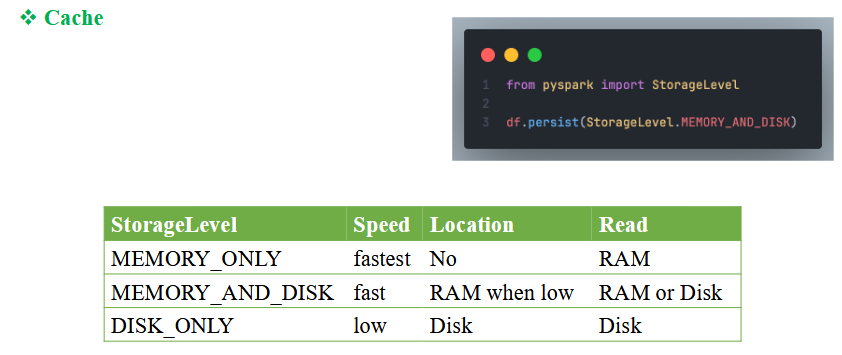
\includegraphics[width=0.7\linewidth]{spark_StorageLevel.png}
    \caption{PySpark Storage Optimization with Stoage Level}
\end{figure}


\begin{itemize}
    \item \textbf{Cache:} Lưu dữ liệu vào RAM (\texttt{MEMORY\_ONLY}) — phù hợp cho dữ liệu vừa khít bộ nhớ.
    \item \textbf{Persist:} Cho phép chọn \textbf{Storage Level} (ví dụ: \texttt{MEMORY\_AND\_DISK}, \texttt{DISK\_ONLY}) — dùng khi dữ liệu quá lớn để lưu toàn bộ trong RAM.
\end{itemize}
\noindent
Thực tế: \texttt{Cache()} chính là \texttt{Persist()} với mặc định \texttt{MEMORY\_ONLY}.


\textbf{Checkpoint} được sử dụng khi:
\begin{itemize}
    \item DAG quá dài, gây rủi ro mất dữ liệu lineage khi node bị lỗi.
    \item Cần lưu trạng thái trung gian đáng tin cậy xuống HDFS hoặc storage ổn định.
\end{itemize}
Khác với Cache/Persist (lưu tạm thời trong bộ nhớ hoặc ổ đĩa local), Checkpoint sẽ ghi dữ liệu xuống hệ thống lưu trữ bền vững (thường là HDFS).

\section{Phần 4: So sánh workflow của Sklearn và PySpark để dễ hiểu hơn}
\textbf{Sklearn}
\begin{figure}[H]
    \centering
    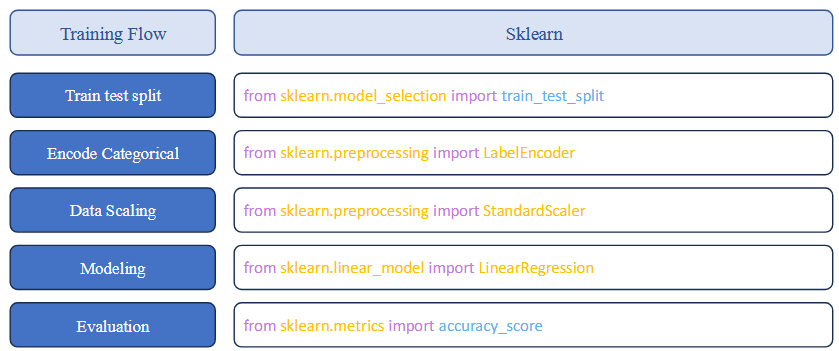
\includegraphics[width=0.7\linewidth]{sklearnFlow.png}
    \caption{Sklearn Training workflow}
\end{figure}


\textbf{PySpark}
\begin{figure}[H]
    \centering
    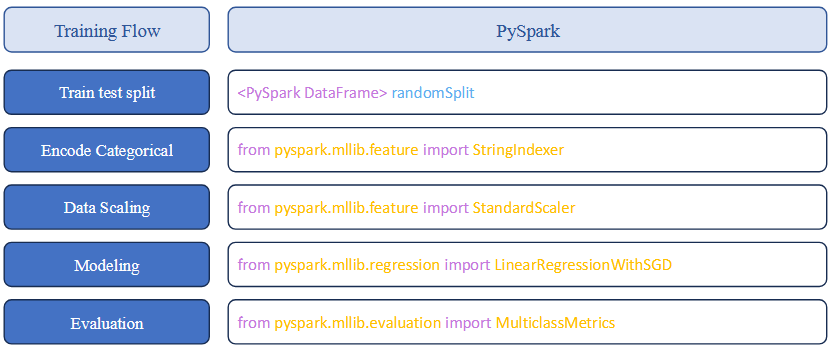
\includegraphics[width=0.7\linewidth]{pysparkFlow.png}
    \caption{Pyspark Training workflow}
\end{figure}

\printbibliography
\end{document}